% !TeX program = xelatex
% Compile from this directory with the three figure*.pdf files beside this source.
\documentclass[aspectratio=169,11pt]{beamer}
\usepackage{fontspec}
\setsansfont{cmunss.otf}[BoldFont=cmunsx.otf,ItalicFont=cmunsi.otf]
\setmainfont{cmunrm.otf}[BoldFont=cmunbx.otf,ItalicFont=cmunti.otf]
\usepackage[main=russian,english]{babel}
\usepackage{amsmath,amssymb,mathtools}
\usepackage{booktabs}
\usepackage{graphicx}
\usefonttheme{serif}

\definecolor{ink}{HTML}{1D2833}
\definecolor{accent}{HTML}{224E73}
\definecolor{muted}{HTML}{64717C}
\setbeamercolor{background canvas}{bg=white}
\setbeamercolor{normal text}{fg=ink}
\setbeamercolor{frametitle}{fg=ink}
\setbeamercolor{structure}{fg=accent}
\setbeamercolor{alerted text}{fg=accent}
\setbeamerfont{frametitle}{size=\Large,series=\bfseries}
\setbeamerfont{title}{size=\LARGE,series=\bfseries}
\setbeamertemplate{navigation symbols}{}
\setbeamertemplate{itemize items}[circle]
\setbeamertemplate{footline}{\hfill{\color{muted}\scriptsize\insertframenumber/\inserttotalframenumber}\hspace{0.5cm}\vspace{0.25cm}}
\setbeamertemplate{frametitle}{\vspace{0.18cm}\insertframetitle\par\vspace{0.18cm}}
\setbeameroption{hide notes}

\newcommand{\figcite}[1]{{\color{muted}\scriptsize Strens (2003), рис.~#1. Оригинальный график.}}
\newcommand{\paperurl}{https://cdn.aaai.org/ICML/2003/ICML03-096.pdf}

\title{Эволюционный MCMC в дискретных пространствах}
\subtitle{Evolutionary MCMC Sampling and Optimization in Discrete Spaces}
\author{Udeneev Alexandr}
\date{Сентябрь 2026}

\begin{document}

% 1 — 0:30
\begin{frame}[plain]
  \vspace{1.3cm}
  {\usebeamerfont{title}\inserttitle\par}
  \vspace{0.28cm}
  {\large\color{accent}\insertsubtitle\par}
  \vspace{0.22cm}
  {\large Malcolm J. A. Strens, ICML 2003\par}
  \vfill
  \insertauthor\hfill\insertdate
  \note{0:30. Представить работу и основной вопрос: можно ли использовать генетические операторы для корректного семплирования?}
\end{frame}

% 2 — 0:55
\begin{frame}{Постановка задачи}
  \[
    \mathcal B=\{0,1\}^{m},\qquad
    \pi(b)=P(b\mid D)=\frac{P(D\mid b)P(b)}{Z},
    \qquad Z=P(D).
  \]
  \vspace{0.25cm}
  \begin{itemize}\setlength{\itemsep}{0.3cm}
    \item $b$ кодирует дискретную гипотезу: например, наличие $m$ заболеваний.
    \item Требуется оценивать ожидания по $\pi$, а не только
      $\hat b_{\mathrm{MAP}}=\arg\max_b\pi(b)$.
  \end{itemize}
  \[
    \mathbb E_{\pi}[R(b,u)]
    \approx \frac1S\sum_{s=1}^{S}R(b^{(s)},u),
    \qquad b^{(s)}\sim\pi.
  \]
  \note{0:55. При принятии решений важно усреднение по неопределённости. Нормирующая константа Z неизвестна, но в отношениях вероятностей сократится.}
\end{frame}

% 3 — 1:00
\begin{frame}{Условие корректности MCMC}
  Для симметричного предложения $q(b'\mid b)=q(b\mid b')$:
  \[
    \alpha(b,b')
    =\min\left\{1,\frac{\pi(b')}{\pi(b)}\right\}.
  \]
  Тогда выполняется детальный баланс:
  \[
    \pi(b)q(b'\mid b)\alpha(b,b')
    =\pi(b')q(b\mid b')\alpha(b',b).
  \]
  \vspace{0.2cm}
  Это делает $\pi$ стационарным распределением цепи. Для сходимости из
  любого начального состояния дополнительно нужна достижимость состояний.
  \note{1:00. Показать, что правило Метрополиса принимает улучшение всегда, ухудшение иногда. Детальный баланс отвечает за правильные частоты в пределе.}
\end{frame}

% 4 — 1:00
\begin{frame}{Мутация как базовое предложение}
  Каждый бит меняется независимо с вероятностью $\rho$.
  Если $d_H(b,b')$ — расстояние Хэмминга, то
  \[
    q_M(b'\mid b)
    =\rho^{d_H(b,b')}(1-\rho)^{m-d_H(b,b')}.
  \]
  \vspace{0.12cm}
  \begin{align*}
    d_H(b,b')&=d_H(b',b)
      &&\Longrightarrow\quad q_M(b'\mid b)=q_M(b\mid b'),\\
    0<\rho<1
      &&&\Longrightarrow\quad q_M(b'\mid b)>0\quad\forall\,b,b'.
  \end{align*}
  \vspace{0.1cm}
  Мутация обеспечивает симметричность и эргодичность, но может медленно
  перемещаться между удалёнными областями высокой вероятности.
  \note{1:00. Отличить математическую гарантию от скорости смешивания. Даже простая мутация теоретически может попасть куда угодно, но редко делает полезный дальний ход.}
\end{frame}

% 5 — 1:05
\begin{frame}{Популяция MCMC-цепей}
  Состояние расширенной цепи:
  \[
    \beta=(b_1,\ldots,b_N)\in\mathcal B^N,
    \qquad
    \phi(\beta)=\prod_{i=1}^{N}\pi(b_i).
  \]
  \vspace{0.15cm}
  Если переходы сохраняют $\phi$, то каждая компонента имеет маргинальное
  распределение $\pi$:
  \[
    \sum_{\beta:\,\beta_i=b}\phi(\beta)=\pi(b).
  \]
  \vspace{0.15cm}
  Остальные члены популяции можно использовать для построения предложения
  для $b_i$, если сохранить обратимость перехода.
  \note{1:05. Не нужно считать цепи независимыми в процессе работы. В равновесии у каждой компоненты правильная маргинальная плотность.}
\end{frame}

% 6 — 1:10
\begin{frame}{XOR-предложение}
  Выбираем разные индексы $i,j,k$ и предлагаем
  \[
    b_i'=b_i\oplus(b_j\oplus b_k).
  \]
  Обозначим маску $d=b_j\oplus b_k$. Тогда
  \[
    b_i'=b_i\oplus d,\qquad
    b_i'\oplus d=b_i.
  \]
  \vspace{0.2cm}
  Следовательно, при фиксированных $j,k$ прямое и обратное предложения
  имеют одинаковую вероятность. Меняются именно координаты, по которым
  $b_j$ и $b_k$ различаются.
  \note{1:10. Это дискретный аналог differential evolution: разность между двумя образцами переносится на третий. Обратимость следует из x xor d xor d = x.}
\end{frame}

% 7 — 0:55
\begin{frame}{XOR: небольшой пример}
  \[
    \begin{array}{rcl}
      b_j&=&\mathtt{111000}\\
      b_k&=&\mathtt{101010}\\ \hline
      d=b_j\oplus b_k&=&\mathtt{010010}
    \end{array}
    \qquad
    \begin{array}{rcl}
      b_i&=&\mathtt{101100}\\
      d&=&\mathtt{010010}\\ \hline
      b_i'=b_i\oplus d&=&\mathtt{111110}
    \end{array}
  \]
  \vspace{0.4cm}
  Для нового состояния применяется обычное правило Метрополиса:
  \[
    \alpha_X=\min\left\{1,\frac{\pi(b_i')}{\pi(b_i)}\right\}.
  \]
  \note{0:55. Пройти битовую маску. Значение целевой плотности нового кандидата вычисляется один раз.}
\end{frame}

% 8 — 1:10
\begin{frame}{Скрещивание должно менять пару}
  Для выбранной битовой маски $s$ два родителя обмениваются битами,
  получая $(c_1,c_2)$. Тот же обмен восстанавливает родителей.
  \[
    (b_i,b_j)\ \overset{s}{\longleftrightarrow}\ (c_1,c_2).
  \]
  Правило принятия для расширенной цепи:
  \[
    \alpha_C
    =\min\left\{
      1,\frac{\pi(c_1)\pi(c_2)}
              {\pi(b_i)\pi(b_j)}
    \right\}.
  \]
  \vspace{0.18cm}
  Один переход скрещивания требует двух новых вычислений $\pi$.
  Замена только одного родителя нарушила бы обратимость этой схемы.
  \note{1:10. В обычном генетическом алгоритме можно просто заменить одной новой строкой старую. Для MCMC такая операция здесь не подходит.}
\end{frame}

% 9 — 1:00
\begin{frame}{Смесь операторов и бюджет вычислений}
  На каждом шаге выбирается предложение $M$, $C$ или $X$.
  \[
    p_M+p_C+p_X=1,\qquad p_M>0.
  \]
  \vspace{0.15cm}
  \begin{center}
  \begin{tabular}{lccc}
    \toprule
    Схема в статье & $p_M$ & $p_C$ & $p_X$\\
    \midrule
    Только мутация & $1$ & $0$ & $0$\\
    Мутация + скрещивание & $2/3$ & $1/3$ & $0$\\
    Мутация + XOR & $1/2$ & $0$ & $1/2$\\
    \bottomrule
  \end{tabular}
  \end{center}
  \vspace{0.2cm}
  Вероятности выбраны так, чтобы поровну разделить бюджет вычислений
  целевой плотности между операторами в каждой смешанной схеме.
  \note{1:00. Для crossover одна попытка стоит вдвое дороже. Поэтому сравнивать только количество итераций было бы нечестно.}
\end{frame}

% 10 — 1:10
\begin{frame}{Тестовая модель QMR-DT}
  Для болезни $b_l\in\{0,1\}$ и признака $f_i\in\{0,1\}$:
  \[
    P(f_i=1\mid b)
    =1-(1-q_{i0})\prod_{l=1}^{m}(1-q_{il})^{b_l}.
  \]
  Независимый априорный закон:
  \[
    P(b)=\prod_{l=1}^{m}p_l^{b_l}(1-p_l)^{1-b_l}.
  \]
  \vspace{0.05cm}
  В эксперименте $m=20$ болезней, $n=80$ признаков и 40 случайно
  сгенерированных задач. Для проверки точные маргинальные вероятности
  вычислялись перебором всех $2^{20}$ состояний.
  \note{1:10. q_i0 — фоновая вероятность признака, q_il — связь болезни с признаком. Подчеркнуть синтетическую природу эксперимента.}
\end{frame}

% 11 — 0:55
\begin{frame}{Что автор называет ошибкой}
  Для каждой болезни $l$:
  \[
    \mu_l=P(b_l=1\mid f),\qquad
    \psi_l=\text{доля выборки с }b_l=1.
  \]
  Мера качества на графиках:
  \[
    E(\mu,\psi)
    =\sum_{l=1}^{m}
      (\mu_l-\psi_l)
      \bigl(\log_2\mu_l-\log_2\psi_l\bigr).
  \]
  \vspace{0.1cm}
  $E=0$ при совпадении маргинальных вероятностей; меньшее $E$ означает
  более точную выборку. Это \emph{ошибка оценки вероятностей}, а не loss
  обучения модели.
  \note{0:55. Объяснить, что показаны ошибки маргинальных вероятностей 20 болезней, а не ошибка классификатора или клиническая точность.}
\end{frame}

% 12 — 1:15
\begin{frame}{Результат: сравнение предложений}
  \begin{center}
    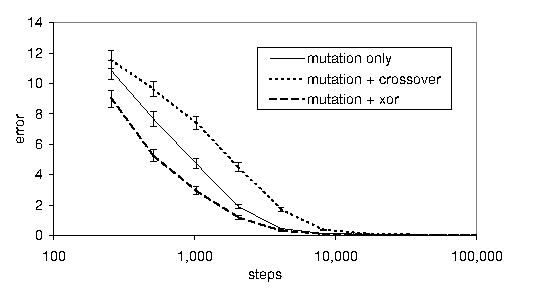
\includegraphics[width=0.94\linewidth,height=0.66\textheight,keepaspectratio]{figure2_error_comparison.pdf}
  \end{center}
  \vspace{-0.18cm}
  {\small На 1024 шагах XOR снижает ошибку на 38\% относительно одной мутации;
  скрещивание увеличивает ошибку.}\\
  \figcite{2}
  \note{1:15. По оси x число вычислений целевой плотности, логарифмическая шкала. Вертикальные отрезки — стандартные ошибки по 40 задачам. Crossover ухудшил результат при том же бюджете.}
\end{frame}

% 13 — 1:00
\begin{frame}{Длительный запуск}
  \begin{center}
    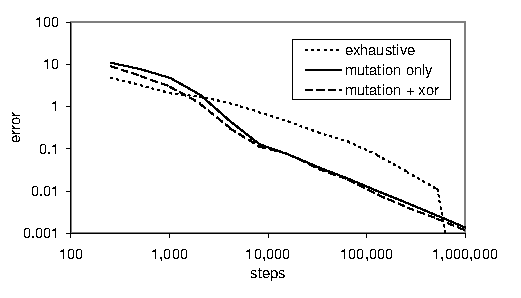
\includegraphics[width=0.94\linewidth,height=0.66\textheight,keepaspectratio]{figure3_long_run.pdf}
  \end{center}
  \vspace{-0.18cm}
  {\small При большом бюджете мутация догоняет XOR; перебор всех состояний
  достигает нулевой ошибки только после $2^{20}$ шагов.}\\
  \figcite{3}
  \note{1:00. Обе оси логарифмические. В начале XOR помогает быстрее исследовать области высокой вероятности; позднее преимущество сокращается.}
\end{frame}

% 14 — 0:55
\begin{frame}{Размер популяции}
  \begin{center}
    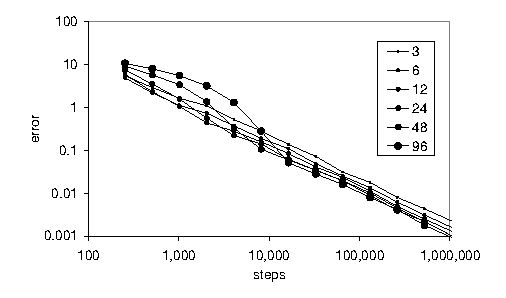
\includegraphics[width=0.94\linewidth,height=0.66\textheight,keepaspectratio]{figure4_population.pdf}
  \end{center}
  \vspace{-0.18cm}
  {\small На раннем этапе из проверенных размеров лучший баланс дал $N=12$.
  После примерно $10^4$ шагов различия уменьшаются.}\\
  \figcite{4}
  \note{0:55. Не утверждать, что N=12 универсален. Большая популяция разнообразнее, но каждый её элемент обновляется реже.}
\end{frame}

% 15 — 0:55
\begin{frame}{Оптимизация через имитацию отжига}
  Если $E(b)$ — функция потерь оптимизации, то
  \[
    \pi_T(b)\propto \exp\!\left(-\frac{E(b)}{T}\right),
    \qquad T\downarrow 0.
  \]
  При охлаждении масса распределения сосредоточивается около глобальных
  минимумов $E$.
  \vspace{0.25cm}

  Проверка в статье: задача восьми ферзей, 24 бита,
  $N=24$, $2^{16}$ шагов; решение находилось с вероятностью $>0{,}99$.
  Все три варианта предложений достигли этого уровня.
  \note{0:55. Здесь метод используется уже как оптимизатор. Опыт с ферзями не демонстрирует особого преимущества XOR.}
\end{frame}

% 16 — 0:45
\begin{frame}{Итог и ограничения}
  \begin{itemize}\setlength{\itemsep}{0.28cm}
    \item Мутация обеспечивает достижимость, а правило Метрополиса сохраняет
      нужное стационарное распределение.
    \item XOR использует различия внутри популяции для более эффективных
      предложений на рассмотренных задачах.
    \item Эксперименты ограничены двоичными строками фиксированной длины и
      синтетической моделью диагностики.
  \end{itemize}
  \vfill
  {\scriptsize Malcolm J. A. Strens. \emph{Evolutionary MCMC Sampling and Optimization in Discrete Spaces}. ICML, 2003.\\
  \url{\paperurl}}
  \note{0:45. Главное: корректность MCMC отдельно от эмпирической скорости смешивания. Открыть вопросы.}
\end{frame}

\end{document}
